\documentclass[dvipsnames,12pt]{beamer}
\usepackage{amsmath,amssymb}
\usepackage{amsfonts}
\usepackage{colortbl}
\usepackage[english]{babel}
\usepackage[brazil]{varioref}
\usepackage{xspace}
\usepackage{cmap}				% Mapear caracteres especiais no PDF
\usepackage{lmodern}
\usepackage[utf8]{inputenc}
\usepackage{epstopdf}
\usepackage{ragged2e}
\usepackage{graphics}
\usepackage{wasysym}
\usepackage{ucs}
\usepackage{pgf}
\usepackage{verbatim}
\usepackage{enumerate}
\usepackage{float, subfigure, multicol, xspace, fancyhdr, wasysym,url}
\usepackage[export]{adjustbox}  % Ajusta o alinhamento entre as figuras
% % TM MARK
% \usepackage{textcomp}
\usepackage{multirow}
% PGFPlot packages
\usepackage{tikz} % Pacotes para plotar gráficos a partir de arquivos de texto
\usepackage{transparent}
\usepackage{mathpazo}

\usepackage{pgfplots}
\usepackage{pgfplotstable}
\usepackage{siunitx}
% \usepgfplotslibrary{external}
%\tikzexternalize[prefix=TikzPictures/] % activate externalization!
\pgfplotsset{compat=newest} % Allows to place the legend below plot
\usepgfplotslibrary{units} % Allows to enter the units nicely
\sisetup{
  round-mode          = places,
  round-precision     = 2,
}
\usepackage{tabularx}
\newcolumntype{C}{>{\centering\arraybackslash}X}
\renewcommand{\arraystretch}{1.2}
\usepackage{circuitikz}
\newcommand{\derivOne}[2]{\dfrac{\partial #1}{\partial #2}}

\mode<presentation> {\usetheme{LVA}}
% \mode<presentation> {\usetheme{CambridgeUS}}
\usecolortheme{orchid}
% Tira os símbolos de navegação
\setbeamertemplate{navigation symbols}{}
% Enumera as figuras
\setbeamertemplate{caption}[numbered]

\makeatletter
\newenvironment{noheadline}{
    \setbeamertemplate{headline}{}
    \addtobeamertemplate{frametitle}{\vspace*{-0.9\baselineskip}}{}
}{}
\makeatother



% \usetikzlibrary{shapes.geometric, arrows}
% \tikzstyle{startstop} = [rectangle, rounded corners, minimum width=3cm, minimum height=1cm,text centered, draw=black, fill=darkblue!30]
% \tikzstyle{arrow} = [thick,->,>=stealth]
%\setbeamertemplate{caption}[numbered]

% \usefonttheme[onlymath]{serif}

\providecommand{\sin}{} \renewcommand{\sin}{\hspace{2pt}\mathrm{sen}}		% Redefine a escrita do seno
\providecommand{\tan}{} \renewcommand{\tan}{\hspace{2pt}\mathrm{tg}}		% Redefine a escrita da tangente


%%%%%%%%%%%%%%%%%%%%%%%%%%%%%%%%%%%%%%%%%%%%%%%%%%%%%%%%%%%%%%%%%%%%%
\title[Laboratory of Acoustic and Vibrations]{Numerical investigation of normal mode radiation properties of ducts with low Mach number inlet flow}
\author[André Loch Gesig]{André Gesing*; Diego Calero, Bernardo Murta, Stephan Paul; Julio Cordioli}
\institute[LVA-UFSC]{Laboratory of Acoustic and Vibrations - Federal University of Santa Catarina}
\date{}
% \date{Buenos Aires, September, 2016}
 %\titlegraphic{
\includegraphics[width=0.8\linewidth,valign=m]{./Figures/ICA_footer.pdf}}
%               \includegraphics[scale=0.45,valign=m]{./Figures/otovidalogo}~\hfill
% 			  
\includegraphics[scale=0.20,valign=m]{./Figures/LVA_Logo.pdf}~\hfill
% 			  \includegraphics[scale=0.27,valign=m]{./Figures/wavetechlogo}~\hfill
% 			  \includegraphics[scale=0.30,valign=m]{./Figures/finep}}
%%%%%%%%%%%%%%%%%%%%%%%%%%%%%%%%%%%%%%%%%%%%%%%%%%%%%%%%%%%%%%%%%%%%%

%% Lista de novos comandos
\newcommand\etal{\textit{et al.}\xspace}

\newcommand{\fig}[1]{Figura~\ref{#1}\xspace}
\newcommand{\figs}[2]{Figuras~\ref{#1}~e~\ref{#2}\xspace}
%%%%%%%%%%%%%%%
%%%%%%%%%%%%%%%%
\newcommand{\tab}[1]{Tabela~\ref{#1}\xspace}
\newcommand{\tabs}[1]{Tabelas~\ref{#1}\xspace}
%%%%%%%%%%%%%%%
%%%%%%%%%%%%%%%%
% % % % % % % % % % % % % % % % % % % % % % % % % % % % % % % % % % % % % % % % % %

\begin{document}
\section*{}
\begin{noheadline}

\setbeamertemplate{footline}{} 

\begin{frame}
  
   \titlepage
   
\end{frame}

\addtocounter{framenumber}{-1}

\end{noheadline}

% \begin{frame}
%   \frametitle{Sumário}
%   \tableofcontents[section=1,hidesubsections]
% \end{frame}


\AtBeginSection[]
{
  \frame<handout:0>
  {
    \frametitle{Summary}
    \setbeamertemplate{footline}{} 
    \tableofcontents[currentsection,hideallsubsections]
  }
}

\AtBeginSubsection[]
{
  \frame<handout:0>
  {
    \frametitle{Sumário}
    \tableofcontents[sectionstyle=show/hide,subsectionstyle=show/shaded/hide]
  }
}

\newcommand<>{\highlighton}[1]{%
  \alt#2{\structure{#1}}{{#1}}
}
\newcommand{\icon}[1]{\pgfimage[height=1em]{#1}}

% %%%%%%%%%%%%%%%%%%%%%%%%%%%%%%%%%%%%%%%%%%%%%%%%%%%%%%%%%%%%%%%%%%%%%

\section{Introduction}
\begin{frame}
\frametitle{Totally implantable hearing devices}
\begin{minipage}[t][][t]{0.4\textwidth}
\begin{figure}
  \centering
\includegraphics [width=\linewidth]{Figures/ICtrad}
\caption{Traditional Cochlear implant. Source: \cite{zeng2008}}
\end{figure}
\end{minipage}
\hfill
\begin{minipage}[t]{0.55\textwidth}
\begin{itemize}
    \item \justifying Presence of an external element in hearing aids and cochlear implants (CI)
    \item Totally implantable CI (TICI) and totally implantable hearing devices have been proposed ~\cite{briggs2008}
    \item Hence, Implantable sensor
\end{itemize}
\end{minipage}
\end{frame}


\section{Implantable Sensors}
\begin{frame}
\frametitle{Implantable sensors}
\begin{itemize}
    \item Subcutaneous microphone~\cite{jenkins2007, pulcherio2014} - skin infections, body noise and variable sensitivity - sensitivity equals to 2~mV/Pa at 90~dB SPL at 1~kHz~\cite{zenner2001} \pause
    \item Piezoresistive accelerometer~\cite{park2007} - bandwidth from 900~Hz to 7~kHz, but high power consumption (1~mW) \pause
    \item Capacitive accelerometer~\cite{ko2009,zurcher2007} - limited sensitivity between 2 and 4~kHz, 30 mV/Pa at 94~dB~SPL at 1~kHz, power consumption about 4.5~mW \pause
    \item Piezoelectric accelerometer~\cite{yip2015,beker2013} -  bandwidth from 300~Hz to  6~kHz and sensitivity equals to 10~mV/Pa for 90~dB~SPL at 1~kHz
\end{itemize}
\end{frame}

\begin{frame}
\frametitle{Requirements of totally implantable sensors}
\begin{minipage}[t][][t]{0.4\textwidth}
    \begin{figure}
  \centering
\includegraphics [width=\linewidth]{Figures/ICtrad}
\caption{Traditional Cochlear implant. Source: \cite{zeng2008}}
\end{figure}
\end{minipage}
\hfill
\begin{minipage}[t]{0.55\textwidth}
\begin{itemize}
    \item Appropriate dynamic range has been assumed to be from 40 to 100 dB SPL~\cite{ko2009}.
    \item Bandwidth has been defined as from 100 Hz to 5 kHz
    \item maximum dimension of 2 mm~\cite{sachse2013}
    \item sensor mass must also be less than 10\% of the ossicle's mass to which it will be fixed \pause
\end{itemize}
\end{minipage}
\vskip 0.3cm
To achieve such limitations, fabrication via micro electromechanical systems (MEMS) technology is considered.
\end{frame}

\section{Design}
\begin{frame}
\frametitle{Design of implantable MEMS piezoelectric accelerometer}
\begin{itemize}
    \item Three designs are analysed via Finite element method (FEM)
    \item MEMS fabrication restrictions imposed by Piezoelectric Multi-User MEMS Processes (PiezoMUMPS\texttrademark by MEMSCAP\textregistered) are considered
\end{itemize}

  \begin{figure}[ht!]
  \centering
\includegraphics [width=1\textwidth]{Figures/Figure1.pdf}
\caption{Top view of the different MEMS designs analysed. Design I: trampoline, design II: hexagonal beams with square seismic mass, design III: annular}
\end{figure}
\end{frame}

\section{Lumped parameter models}
\begin{frame}
\frametitle{Lumped parameter model of the middle ear}
    Lumped parameter model was used to represent the coupled system formed by the accelerometer and the ossicles of middle ear~\cite{oconnor2008}.
    \vskip-0.5cm
\begin{figure}[!ht]
\centering
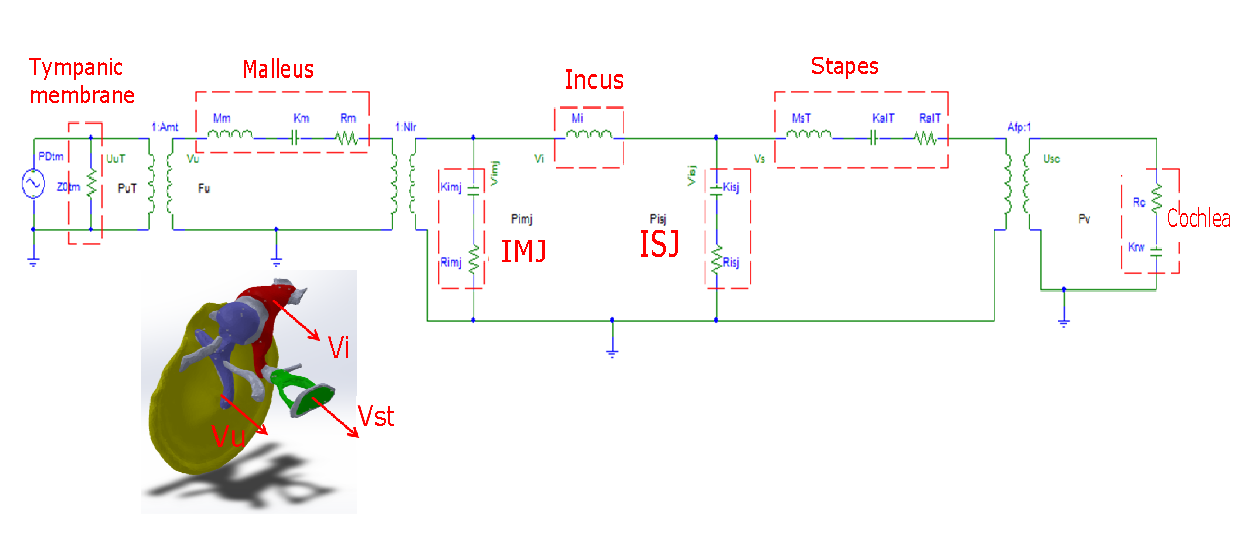
\includegraphics [width=1.05\textwidth]{Figures/Figure2.eps}
%\text{Source: Authors}
\caption{Equivalent circuit model of the middle ear and direction of velocities}
\label{fig:CE_OM3}
\end{figure}
\end{frame}

\begin{frame}
\frametitle{Lumped parameter model of the accelerometer}
\vskip-0.5cm
    Lumped parameter model of the accelerometer and pre-amplifier is coupled to the lumped model of the middle ear.
    \vskip-0.2cm

\begin{figure}[!ht]
\centering
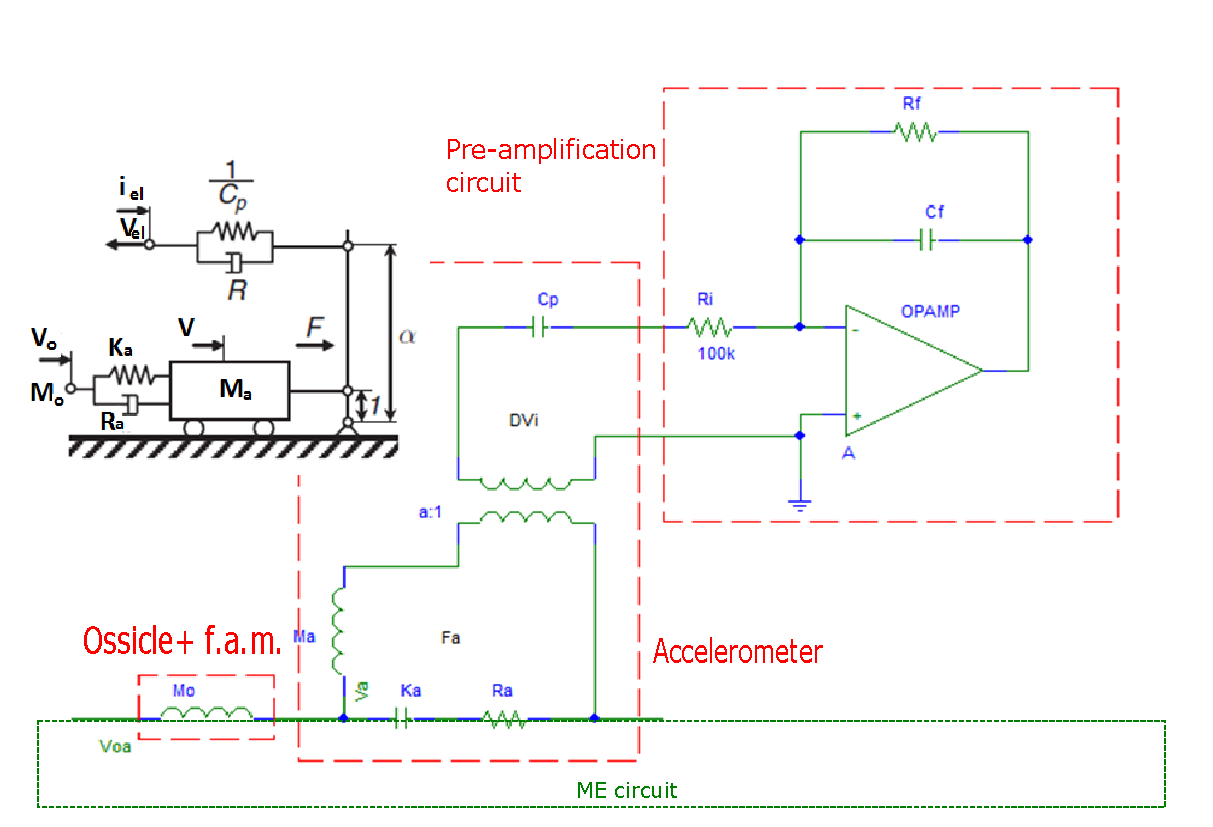
\includegraphics [width=0.8\textwidth]{Figures/Figure3.eps}
%\text{Source:Authors}
\caption{Equivalent circuit model of the accelerometer with its pre-amplification circuit coupled to the ossicular chain}
\label{fig:CE_OM2}
\end{figure}
\end{frame}

\section{Results}
\begin{frame}
\frametitle{Accelerometer response optimization}
    \begin{table}[ht!]
 \caption{Response of optimized MEMS accelerometers.}
    \label{tab:optimized_accelerometer}
    \centering
   \begin{tabularx}{\linewidth}{cCc}
   \hline 
   Design & Natural frequency [kHz] & Charge sensitivity [pC/$g$] \\\hline \hline
         I &  15.4 & 0.048  \\
         II &  10.0 & 0.051  \\
         III & 18.8 & 0.071  \\
          \hline
    \end{tabularx}
\end{table}
  \begin{figure}[ht!]
  \centering
\includegraphics [width=\textwidth]{Figures/Figure1.pdf}
\caption{Design I: trampoline, design II: hexagonal beams with square seismic mass, design III: annular}
\label{fig:types_of_accelerometers}
\end{figure}
\end{frame}


\begin{frame}
\frametitle{Voltage sensitivity of accelerometers}
Voltage responses reach a maximum of 30 mV/Pa at 300 Hz, decaying to 0.7 mV/Pa at 1 kHz.
\vskip-0.6cm
\begin{figure}[!ht]
\begin{center}
\begin{tikzpicture}
\begin{loglogaxis}[
    title={},
    width=\textwidth,
    height=0.5\textwidth,
    xlabel={Frequency},
    ylabel={Voltage sensitivity},
	y unit={mV/Pa},
	x unit=Hz,
     xmin=100, xmax=10000,
    % ymin=0,
    legend pos=north east,
    grid=major, % Display a grid	
	grid style={dashed,gray!30}, % Set the style
	]
     \addplot[color=blue,thick] table[x index=0,y index=3] {Sens_tr.txt}; \label{Trampoline}
     \addlegendentry{I}
     \addplot[color=red,dashed,thick] table[x index=0,y index=3] {Sens_hex.txt}; \label{Hexagonal}
     \addlegendentry{II}
      \addplot[color=black,dotted,thick] table[x index=0,y index=3] {Sens_an.txt}; \label{Annular}
     \addlegendentry{III}
\end{loglogaxis}
\end{tikzpicture}
\caption{Voltage sensitivity of the different designs coupled to the malleus.}
\label{fig:designs_ME}
\end{center}
\end{figure}
\end{frame}

\begin{frame}
 \frametitle{Voltage sensitivity coupled to different ossicles}
  According to this simplified model, malleus and stapes are the best candidates to fix an accelerometer.
  \vskip -0.6cm
 \begin{figure}[!ht]
\begin{center}
\begin{tikzpicture}
\begin{loglogaxis}[
    width=\textwidth,
    height=0.5\textwidth,
    xlabel={Frequency},
    ylabel={Voltage sensitivity},
	y unit={mV/Pa},
	x unit=Hz,
     xmin=100, xmax=10000,
    legend pos=north east,
    grid=major, % Display a grid	
	grid style={dashed,gray!30}, % Set the style
	]
    \addplot[color=blue,dotted,thick] table[x index=0,y index=1] {Sens_tr.txt}; \label{Incus}
    \addlegendentry{Incus}
     \addplot[color=red,thick] table[x index=0,y index=3] {Sens_tr.txt}; \label{Malleus}
     \addlegendentry{Malleus}
      \addplot[color=black,dashed,thick] table[x index=0,y index=5] {Sens_tr.txt}; \label{Stapes}
     \addlegendentry{Stapes}
\end{loglogaxis}
\end{tikzpicture}
\caption{Voltage sensitivity of the design I (trampoline) accelerometer coupled to different ossicles of the middle ear.}
\label{fig:analysis_ME}
\end{center}
\end{figure}
\end{frame}

\section{Conclusions and ongoing work}
\begin{frame}
\frametitle{Conclusions and ongoing work}
\begin{block}{Conclusions}
\begin{itemize}
    \item An approach based on FEM and EC can be applied to investigate the behaviour of an implantable sensor for hearing devices.
    \item Promising results for piezoelectric MEMS accelerometers. Voltage sensitivity equals to 0.7~mV/Pa at 1~kHz (2~mV/Pa in subcutaneous microphone).
    \item Mass of the designed accelerometers vary from 1.9 to 2.3~mg.
\end{itemize}
\end{block}
\end{frame}


\begin{frame}
\frametitle{Conclusions and ongoing work}
\begin{block}{Ongoing work}
\begin{itemize}
    \item Validation of FEM accelerometer models (prototypes will arrive in September 30).
    \item Consideration of amplifier circuit on analysis.
    \item Development of a multibody dynamic system that represents the behaviour of the middle ear more realistically.
\end{itemize}
\end{block}
\end{frame}
\begin{frame}
 
\begin{center}
Thank you!\\[2cm]Questions?
\end{center}
\end{frame}

\begin{frame}[allowframebreaks]{References}
 \bibliographystyle{abbrv}
 
 \renewcommand{\refname}{\normalfont\selectfont\normalsize}
 \justifying
% \noindent \textbf{References}
% \vspace{-1.2cm}
 \begin{thebibliography}{5}
\begin{footnotesize}
\begin{justifying}


\bibitem{briggs2008}
Briggs, R. J.; Eder, H. C.; Seligman, P. M.; Cowan, R. S.; Plant, K. L.; Dalton, J.; Money, D. K. \& Patrick, J. F. Initial clinical experience with a totally implantable cochlear implant research device Otology \& Neurotology, LWW, 2008, 29, 114-119

\bibitem{zeng2008}
Zeng, F.-G.; Rebscher, S.; Harrison, W.; Sun, X. \& Feng, H. Cochlear implants: system design, integration, and evaluation Biomedical Engineering, IEEE Reviews in, IEEE, 2008, 1, 115-142

\bibitem{jenkins2007}
Jenkins, H. A.; Atkins, J. S.; Horlbeck, D.; Hoffer, M. E.; Balough, B.; Arigo, J. V.; Alexiades, G. \& Garvis, W. US Phase I preliminary results of use of the Otologics MET Fully-Implantable Ossicular Stimulator Otolaryngology--Head and Neck Surgery, SAGE Publications, 2007, 137, 206-212

\bibitem{pulcherio2014}
Pulcherio, J. O. B.; Bittencourt, A. G. \& others. Carina and Esteem: A Systematic Review of Fully Implantable Hearing Devices PloS one, Public Library of Science, 2014, 9, e110636


\bibitem{zenner2001}
Zenner, H. P. \& Leysieffer, H. Total implantation of the implex TICA hearing amplifier implant for high-frequency sensorineural hearing loss: the tübingen university experience Otolaryngologic Clinics of North America, Elsevier, 2001, 34, 417-446


\bibitem{park2007}
Park, W.-T.; O'Connor, K. N.; Chen, K.-L.; Mallon Jr, J. R.; Maetani, T. \& others Ultraminiature encapsulated accelerometers as a fully implantable sensor for implantable hearing aids Biomedical microdevices, Springer, 2007, 9, 939-949
\bibitem{ko2009}
Ko, W. H.; Zhang, R.; Huang, P.; Guo, J.; Ye, X.; Young, D. J. \& Megerian, C. A. Studies of MEMS acoustic sensors as implantable microphones for totally implantable hearing-aid systems Biomedical Circuits and Systems, IEEE Transactions on, IEEE, 2009, 3, 277-285

\bibitem{zurcher2007}
Zurcher, M.; Young, D.; Semaan, M.; Megerian, C. \& Ko, W. MEMS middle ear acoustic sensor for a fully implantable cochlear prosthesis Micro Electro Mechanical Systems, 2007. MEMS. IEEE 20th International Conference on, 2007, 11-14

\bibitem{yip2015}
Yip, M.; Jin, R.; Nakajima, H. H.; Stankovic, K. M. \& Chandrakasan, A. P. A Fully-Implantable Cochlear Implant SoC With Piezoelectric Middle-Ear Sensor and Arbitrary Waveform Neural Stimulation IEEE Journal of Solid-State Circuits, IEEE, 2015

\bibitem{beker2013}
Beker, L.; Zorlu, O.; Goksu, N. \& Kulah, H. Stimulating auditory nerve with MEMS harvesters for fully implantable and self-powered cochlear implants Solid-State Sensors, Actuators and Microsystems (TRANSDUCERS \& EUROSENSORS XXVII), 2013 Transducers \& Eurosensors XXVII: The 17th International Conference on, 2013, 1663-1666

\bibitem{sachse2013}
Sachse, M.; Hortschitz, W.; Stifter, M.; Steiner, H. \& Sauter, T. Design of an implantable seismic sensor placed on the ossicular chain Medical engineering \& physics, Elsevier, 2013, 35, 1399-1405


\bibitem{oconnor2008}
O'Connor, K. N. \& Puria, S. Middle-ear circuit model parameters based on a population of human ears The Journal of the Acoustical Society of America, Acoustical Society of America, 2008, 123, 197-211

\end{justifying}

\end{footnotesize}

\end{thebibliography}

\end{frame}

\end{document}


